% !TEX root = ../../../main.tex
% 来源：中学数学实验教材·第一册（代数）
% 章节：一元二次方程 / 平方与平方根
% 原始文件：3.tex，行 719-743
% 类型：tikz
% ---
    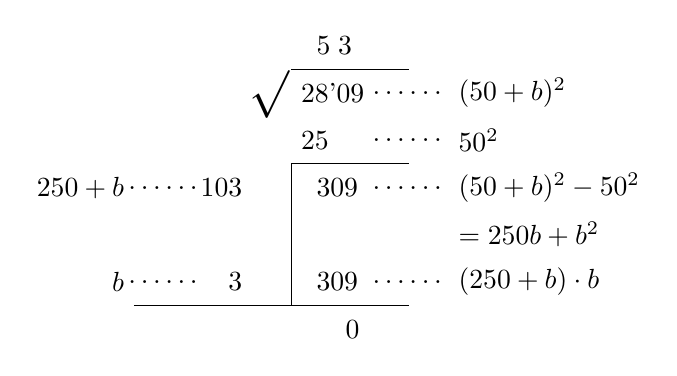
\begin{tikzpicture}[yscale=.6]
    \node at (0,2)[right]{\;\;5\;3};
\node at (0,1)[right]{28'09};  \node at (2,1)[right]{$(50+b)^2$};
\node at (0,0)[right]{25};     \node at (2,0)[right]{$50^2$};
\node at (0,-1)[right]{\;\;309};     \node at (2,-1)[right]{$(50+b)^2-50^2$};    \node at (2,-2)[right]{$=2\x 50\x b+b^2$};   
\node at (-.5,-1)[left]{103};   \node at (-2,-1)[left]{$2\x 50+b$}; 
\node at (.1,1)[left]{\LARGE $\sqrt{}$};

\node at (0,-3)[right]{\;\;309};     \node at (2,-3)[right]{$(2\x 50+b)\cdot b$};
\node at (-.5,-3)[left]{3}; \node at (-2,-3)[left]{$b$};
\node at (0,-4)[right]{\quad\; 0}; 

\draw(0,1.5)--(1.5,1.5);
\draw(0,-3.5)--(0,-.5)--(1.5,-.5);\draw(-2,-3.5)--(1.5,-3.5);

\foreach \x in {1,0,-1,-3}
{
    \node at (1.5,\x){……};
}
\foreach \x in {-1,-3}
{
    \node at (-1.6,\x){……};
}

\end{tikzpicture}
